\documentclass{standalone}
\usepackage{tikz}
\usetikzlibrary{calc}
\begin{document}
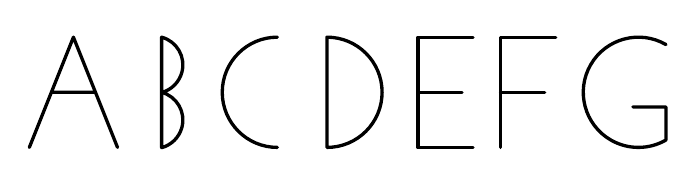
\begin{tikzpicture}[line width=1.2pt, line cap=round, line join=round, scale=1.4]
\def\dx{1.5}

% A
\draw (0,0) -- (0.4,1) -- (0.8,0) (0.2,0.5) -- (0.6,0.5);

% B
\begin{scope}[xshift=0.8*\dx cm]
    \draw (0,0) -- (0,1) arc[start angle=75, end angle=-75, radius=0.26] -- (0,0.5) arc[start angle=75, end angle=-75, radius=0.26] -- (0,0);
\end{scope}

% C
\begin{scope}[xshift=1.5*\dx cm]
    \draw (0,1) arc[start angle=90, end angle=270, radius=0.5];
\end{scope}

% D
\begin{scope}[xshift=1.8*\dx cm]
    \draw (0,0) -- (0,1) arc[start angle=90, end angle=-90, radius=0.5];
\end{scope}

% E
\begin{scope}[xshift=2.35*\dx cm]
    \draw (0.5,0) -- (0,0) -- (0,1) -- (0.5,1) (0,0.5) -- (0.4,0.5);
\end{scope}

% F
\begin{scope}[xshift=2.85*\dx cm]
    \draw (0,0) -- (0,1) -- (0.5,1) (0,0.5) -- (0.4,0.5);
\end{scope}

% G
\begin{scope}[xshift=3.35*\dx cm]
    \draw (0.5,0.5) ++(60:0.5) arc[start angle=60, end angle=300, radius=0.5] -- ++(0,0.3) -- ++(-0.3,0);
\end{scope}
\end{tikzpicture}
\end{document}
